\subsection{LDA Approach} % (fold)
\label{sub:own_lda}

After we developed our pre-processing pipeline for the dataset and some basic analysis on the data we have we decided to use the LDA for a first topic modelling. The LDA approach serves as reference for the result we wanted to obtain by the neural network to have a result for evaluating.


For our LDA approach we used our pre-processed requirements. To apply the LDA we transformed the data in the following way. We created a matrix where each row represents one of the 2966 requirements. the columns are the single words of the requirements. But as the LDA needs a numerical representation of the words we first applied a bag-of-words to the single requirements. As the results were not sufficient we decided to calculate the TF-IDF to get weights for the single words. After these steps we had a prepared matrix that holds the data that now can be used for the LDA.

\begin{figure}[bht]
    \subfigure[LDA Plot with colors to topics\label{fig:lda-tf-idf-topics}]{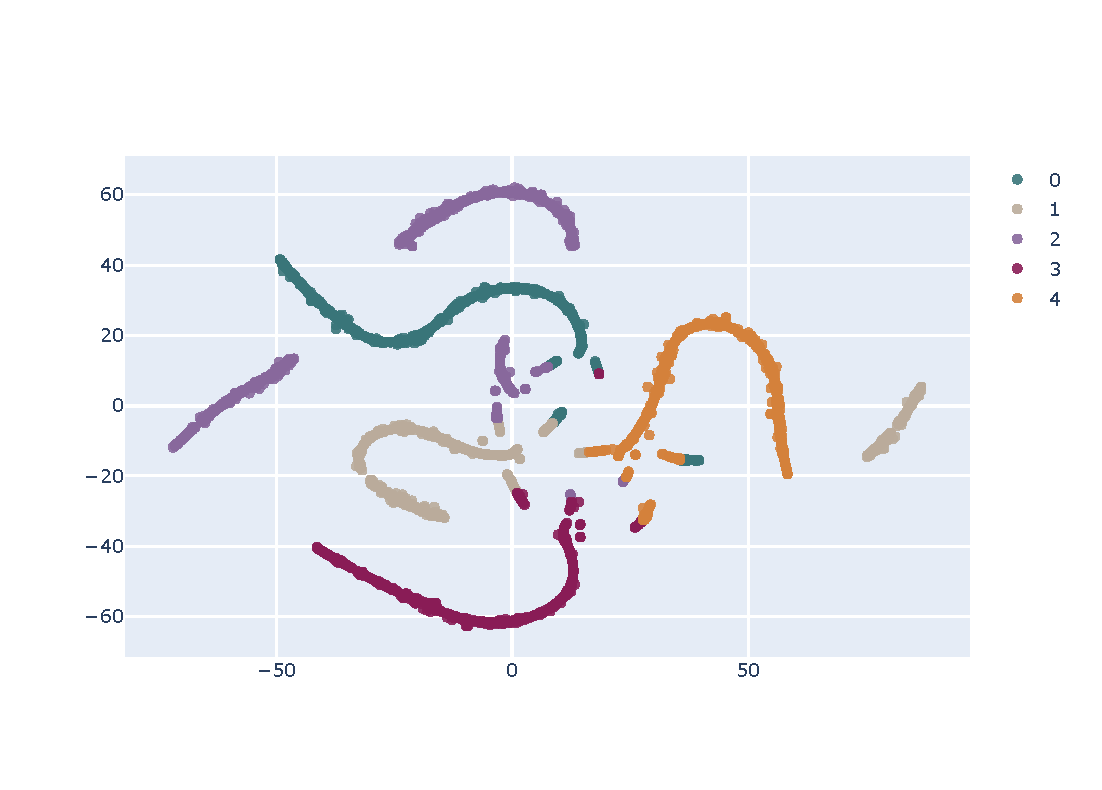
\includegraphics[width=0.49\textwidth]{screenshots/lda-tf-idf.pdf}}
    \subfigure[LDA Plot with colors for domains\label{fig:lda-tf-idf-domains}]{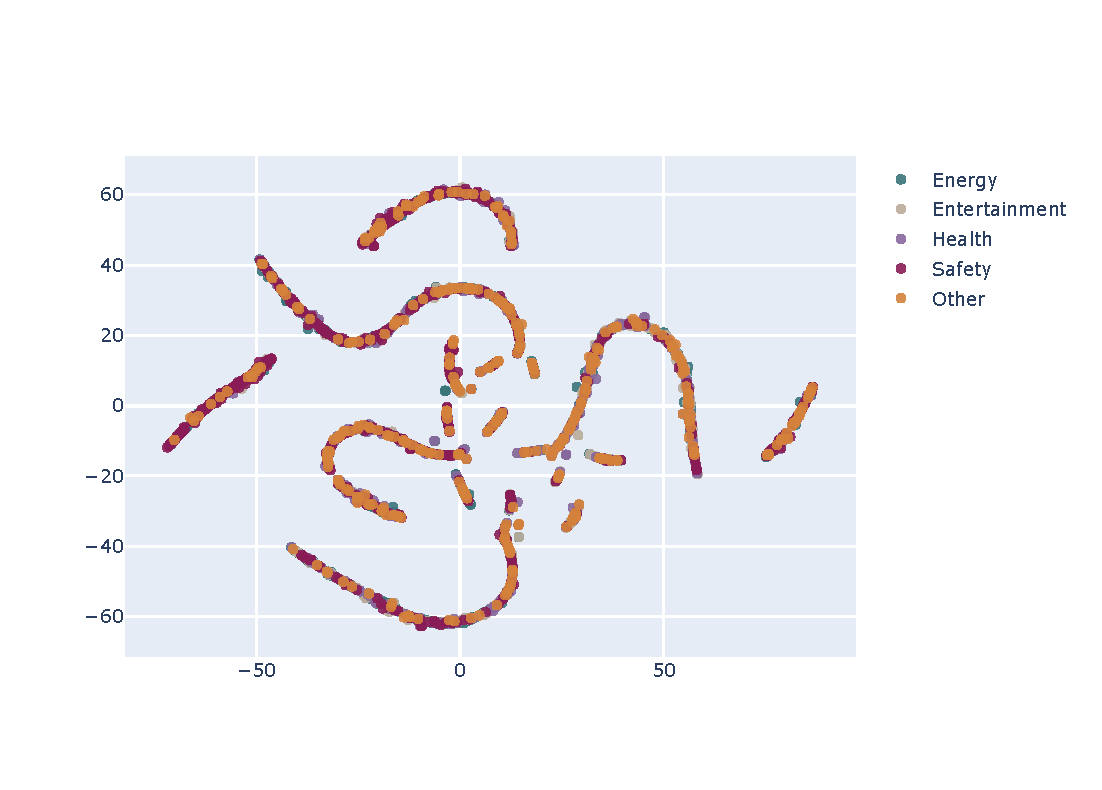
\includegraphics[width=0.49\textwidth]{screenshots/lda-domains.pdf}}
    \caption{LDA Result with TF-IDF (plotted with t-SNE)} \label{fig:lda-tf-idf}
\end{figure}
\FloatBarrier

In \autoref{fig:lda-tf-idf} we can see the two-dimensional representation of the results of the LDA. The reduction of the dimensions is performed by t-SNE which tries to preserve the most differing dimensions. In \autoref{fig:lda-tf-idf-topics} the colors are mapped to the found topics which leads to separable clusters. But if we look for the expected mapping to the domains in \autoref{fig:lda-tf-idf-domains} we can see that the found cluster doesn't represent the expected clusters that where defined by the domains.